 \begin{figure}[tbh]
    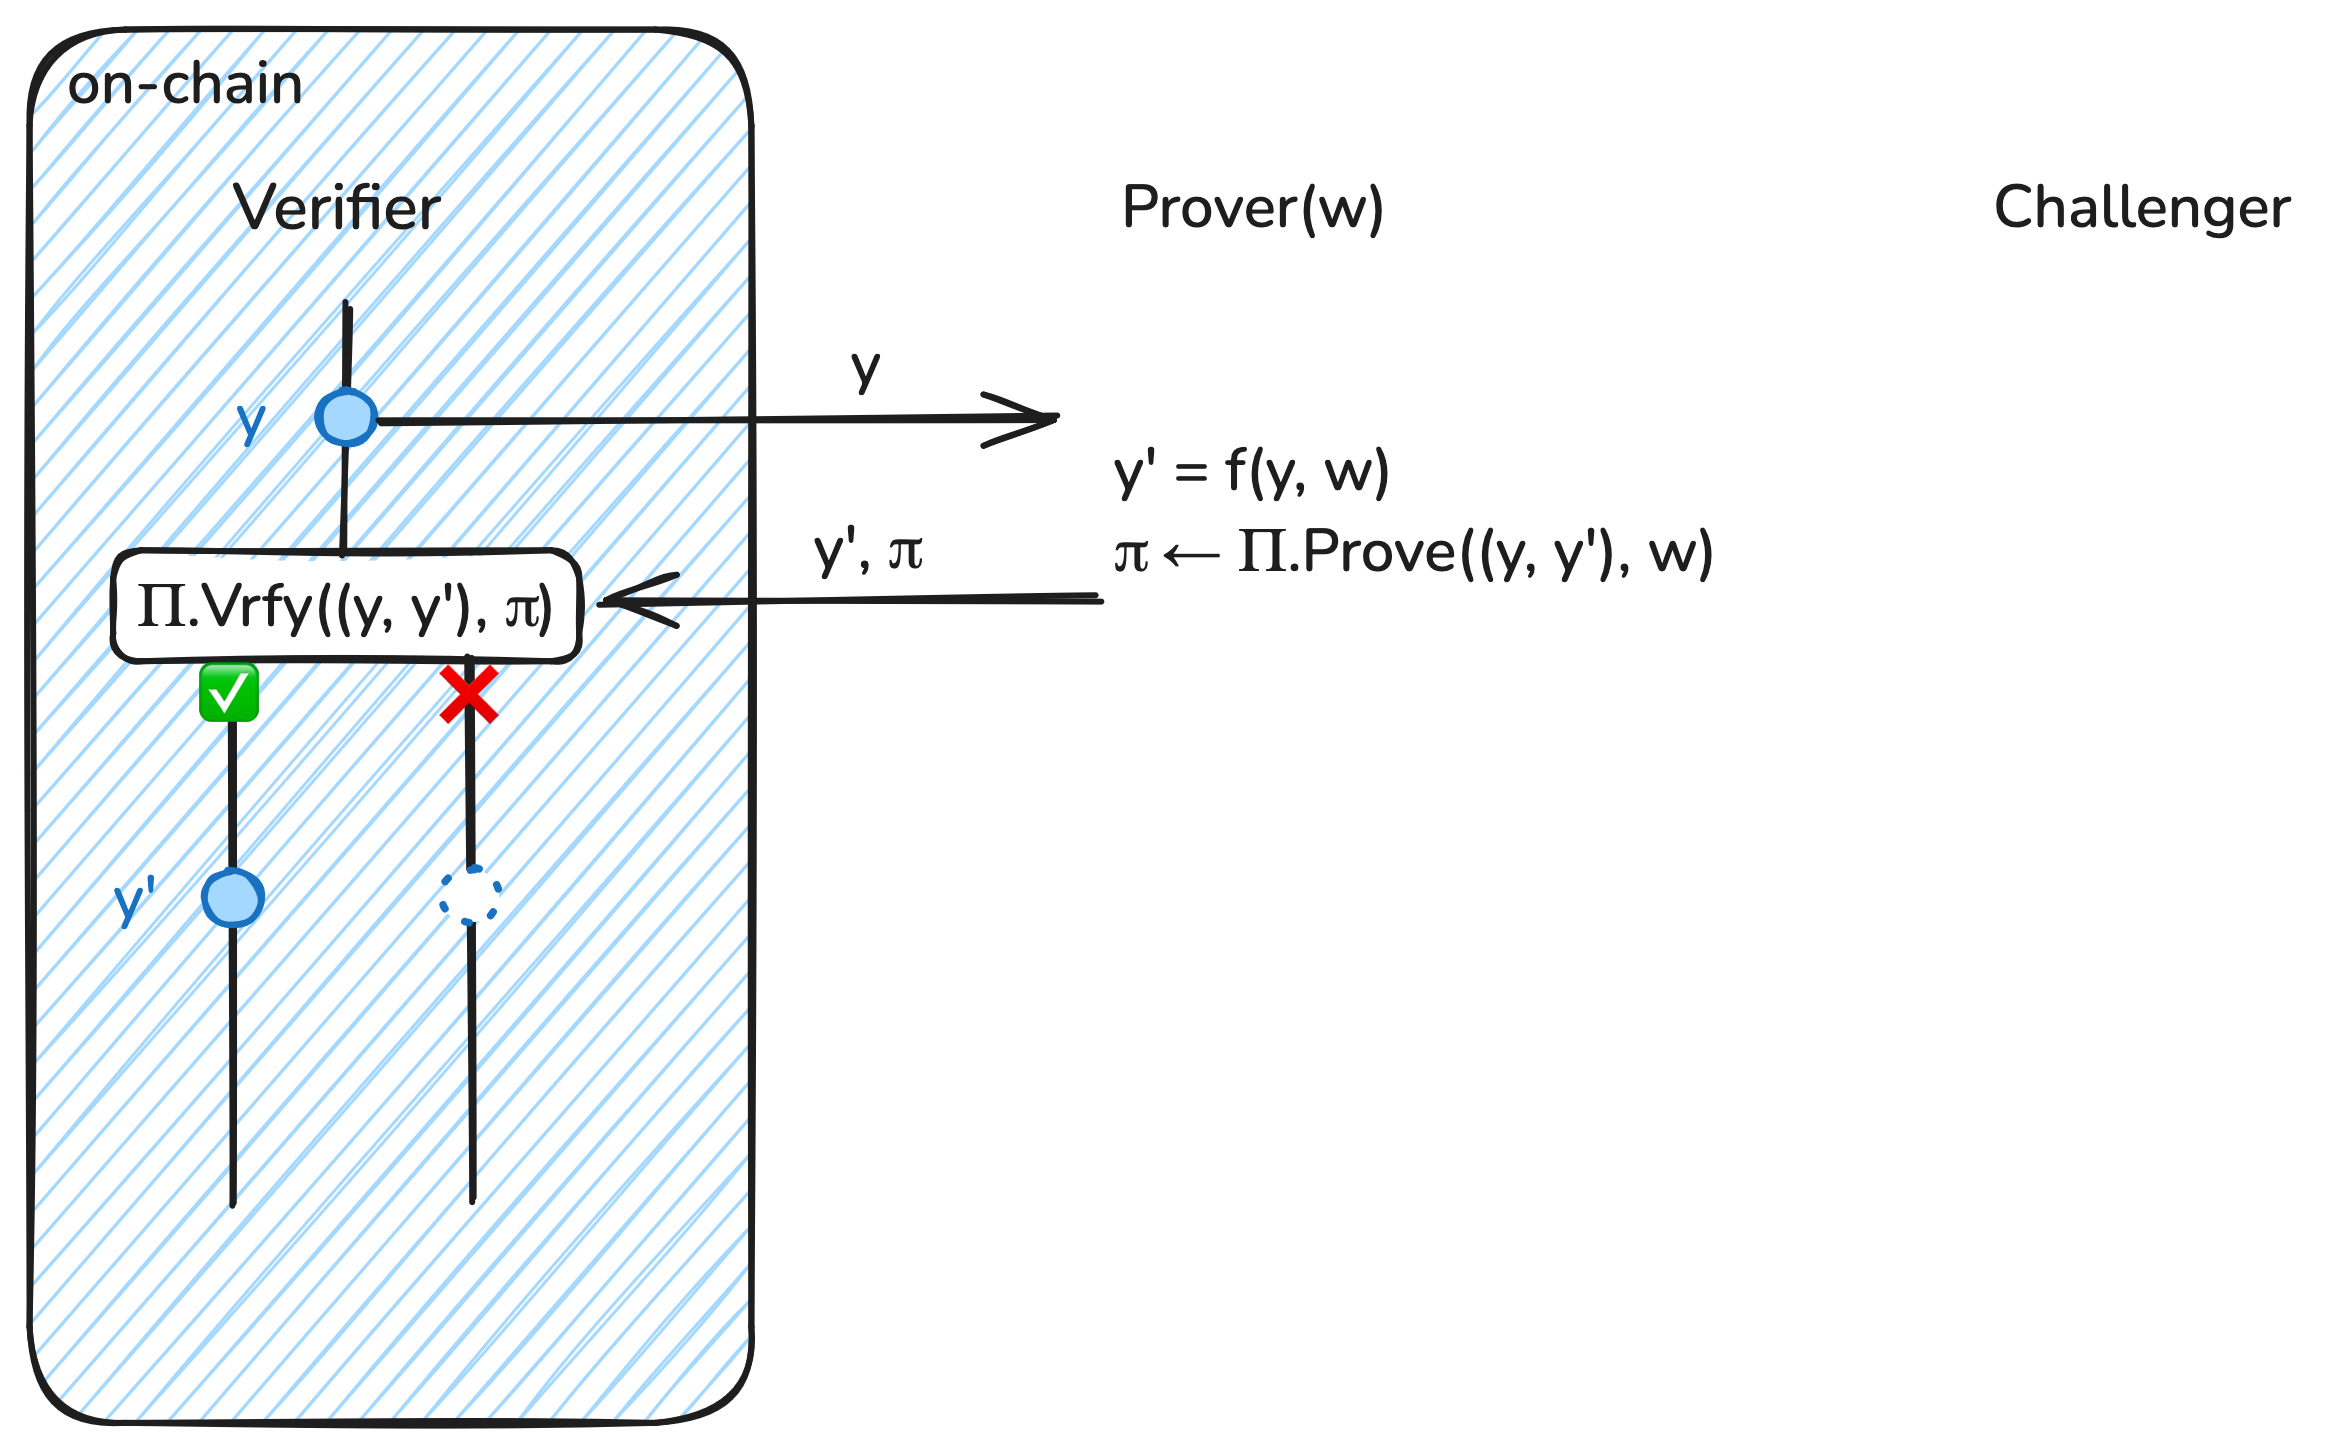
\includegraphics[width=\textwidth]{naysayer/figs/vc.png}
    \caption{\textbf{Using VC to move computation off-chain.} The off-chain ``prover'' applies the function $f$ to input $y$ and potentially auxiliary input $w$ to get the result $y' = f(y, w)$. (In the case of a zk-rollup, $f$ is the state transition function, $y$ is the previous on-chain state, $w$ is a batch of transactions, and $y'$ is the new state after applying the transactions in $w$ to $y$.) It posts $y'$ and a proof $\pi$ of its correctness, which is verified on-chain before the output $y'$ is accepted. This paradigm does not require any challengers.}
    \label{fig:vc}
 \end{figure}

In most blockchains with programming capabilities, e.g., Ethereum~\cite{ethereum_yellowpaper}, developers are incentivized to minimize the storage and computation complexity of on-chain programs. Applications with high compute or storage incur significant fees, commonly referred to as \emph{gas}, to compensate validators in the network. Often, these costs are passed on to users of an application. 

High gas costs have motivated many applications to utilize \emph{verifiable computation (VC)}~\cite{C:GenGenPar10}, off-loading expensive operations to powerful but untrusted off-chain entities who perform arbitrary computation and provide a succinct non-interactive proof (SNARK) that the claimed result is correct.
This computation can even depend on secret inputs not known to the verifier in the case of zero-knowledge proofs (i.e., zkSNARKs).
 %In some cases (though not all), this proof is also zero-knowledge, hiding some inputs to the computation. This is commonly referred to as a \emph{zk-rollup} (even if it is not zero-knowledge).

VC leads to a paradigm in which smart contracts, while capable of arbitrary computation, primarily act as verifiers and outsource all significant computation off-chain (see \Cref{fig:vc}). A motivating application is so-called ``zk''-\emph{rollups}\footnotemark~\cite{starknet,zksync,aztec,dydx,scroll}, which combine transactions from many users into a single smart contract which verifies a proof that all have been executed correctly.
\footnotetext{Note that ``zk-rollup'' is somewhat of a misnomer, since these services do not necessarily meet the zero-knowledge property.} 
However, verifying these proofs can still be costly. For example, the StarkEx rollup 
%contract verifying the state transitions of the off-chain StarkEx marketplace 
has spent hundreds of thousands of dollars to date to verify FRI polynomial commitment opening proofs.\footnote{\url{https://etherscan.io/address/0x3e6118da317f7a433031f03bb71ab870d87dd2dd}}
% Even verifying simple statements can exceed the block gas limit of Ethereum~\cite{EPRINT:NRBB22}\todo{not sure about this example. Maybe a dollar figure on STARKs would more convincing?}\istvan{I had in mind the CRS for EIP-4844 that would have been exceeded the block gas limit with this solution.}.

We observe that this proof verification is often wasteful. In most applications, provers have strong incentives to post only correct proofs, suffering direct financial penalties (in the form of a lost security deposit) or indirect costs to their reputation and business for posting incorrect proofs. As a result, a significant fraction of a typical layer-1 blockchain's storage and computation is expended verifying proofs, which are almost always correct.\footnote{At the time of this writing, we are unaware of any major rollup service which has posted an incorrect proof in production.}

 \begin{figure}[tbh]
    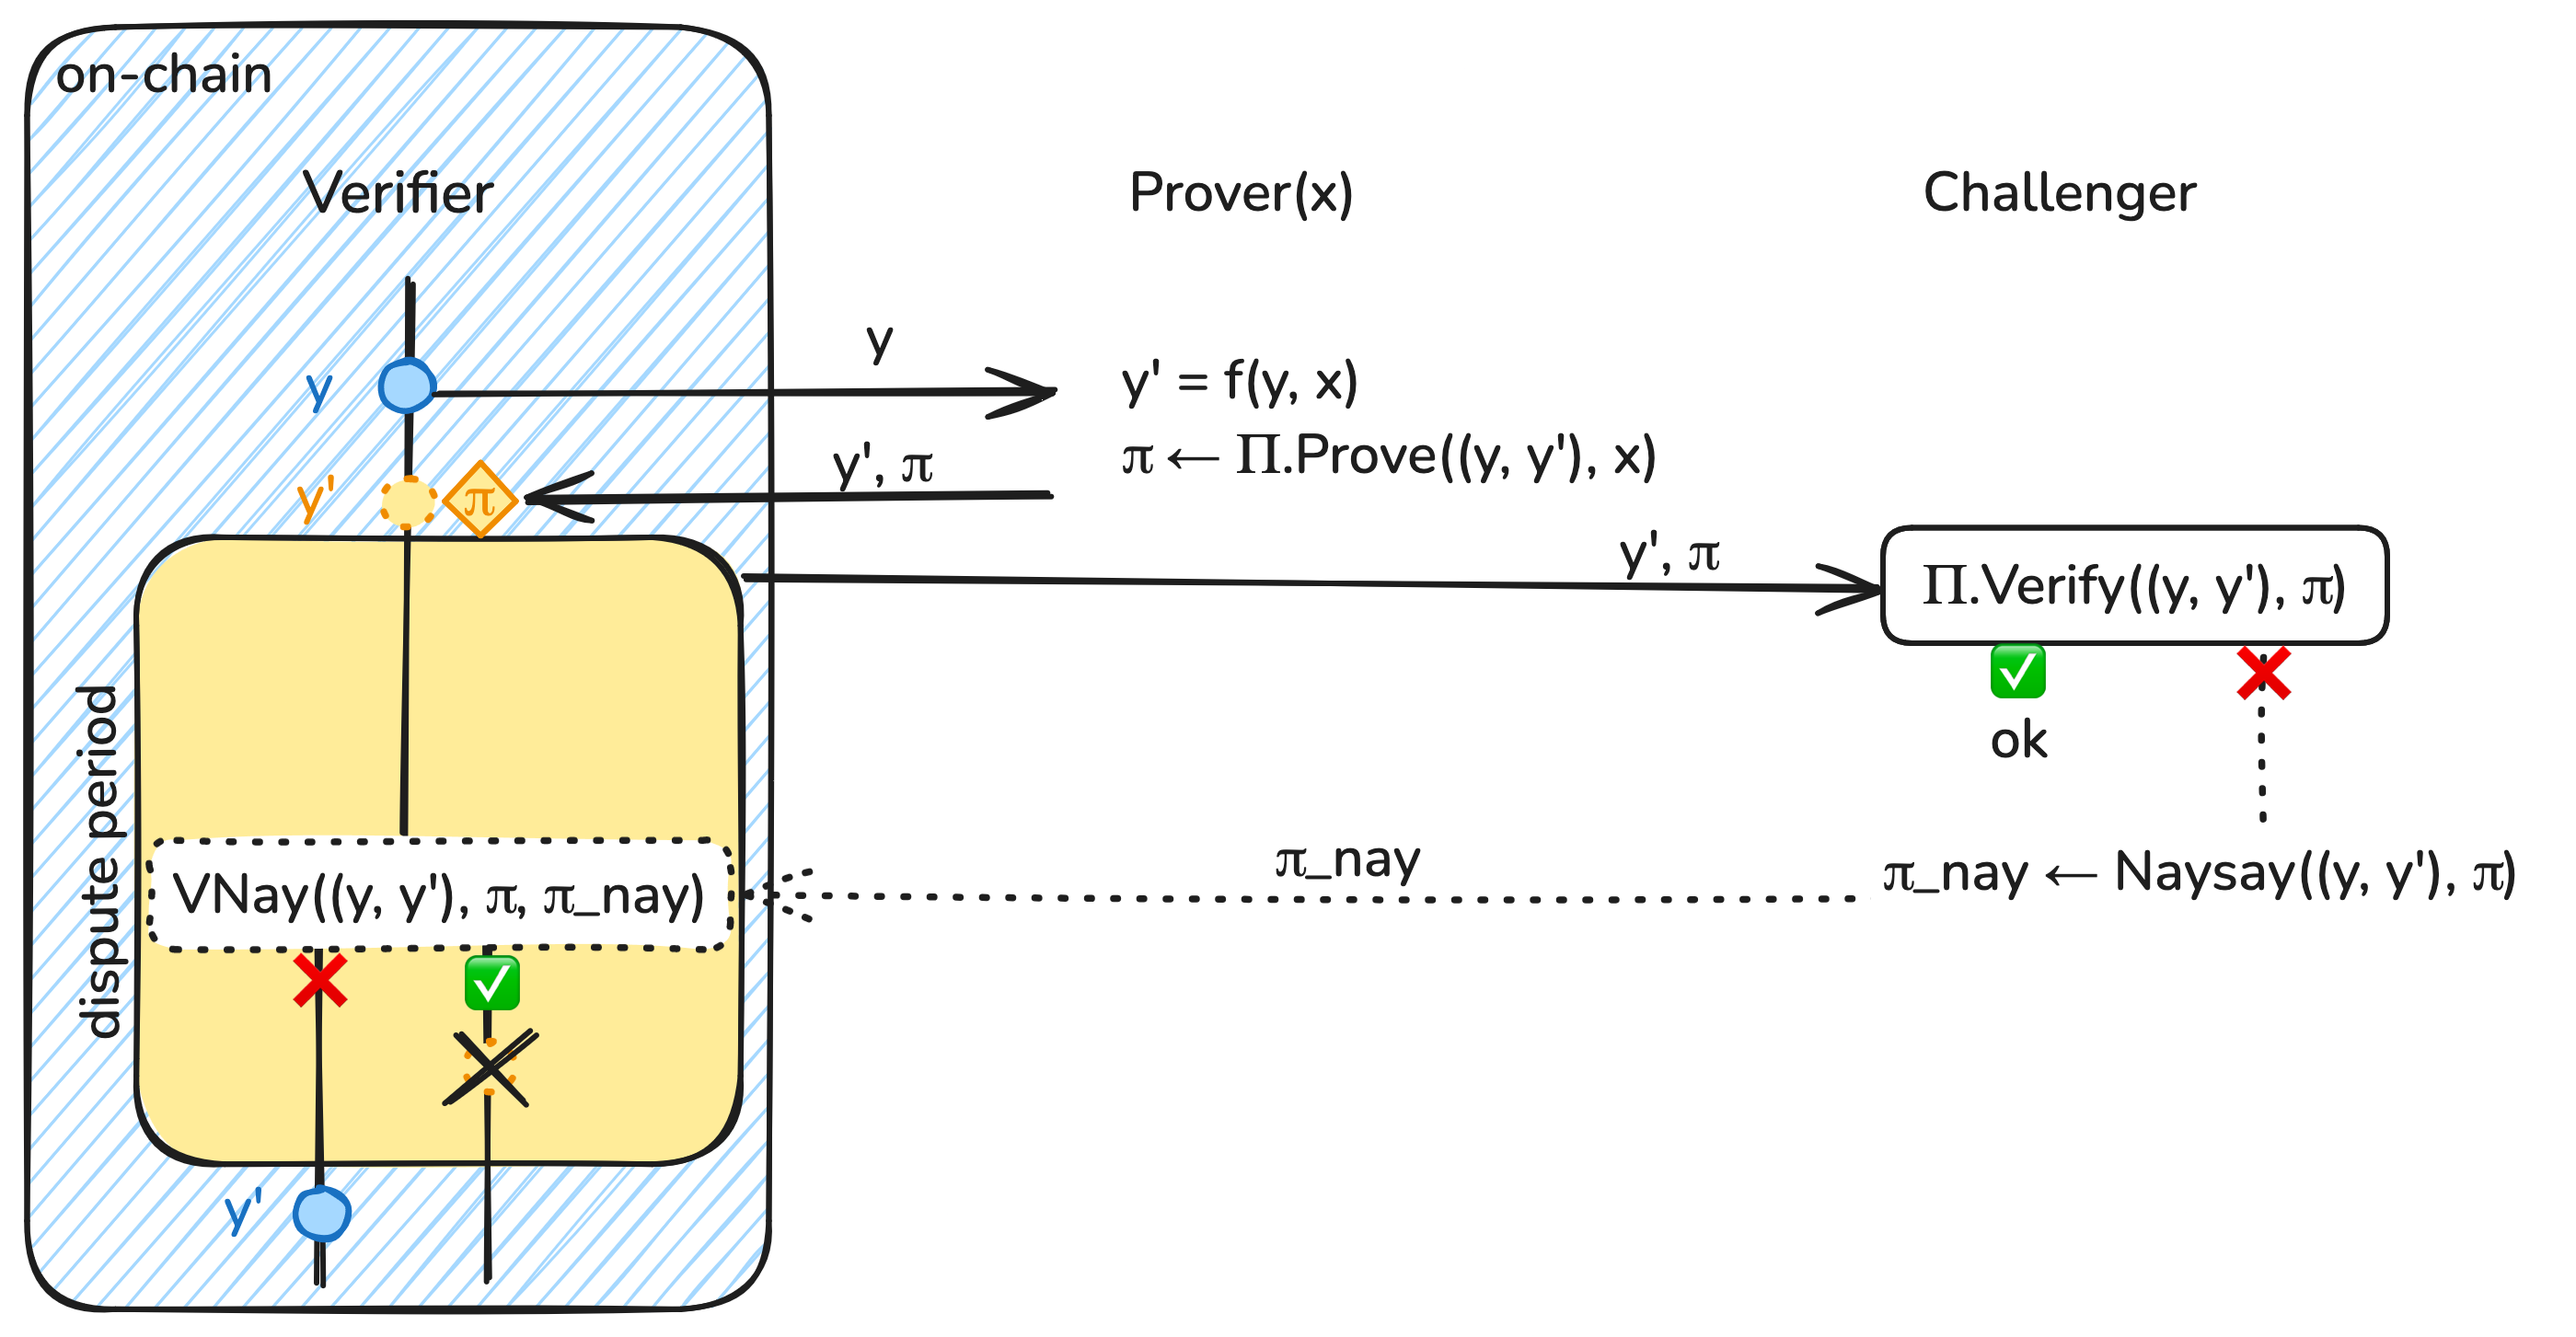
\includegraphics[width=\textwidth]{naysayer/figs/naysayer.png}
    \caption{\textbf{The naysayer proof approach.} As in VC, the off-chain prover computes $y' = f(y, w)$ and $\pi$, which it posts on-chain. This time, the proof is \emph{not} verified on-chain, but is provisionally accepted while waiting for the challenge period to pass. Any party can verify $\pi$ off-chain and, if it fails, issue a challenge by creating a naysayer proof $\pi_\nay$. The on-chain verifier checks any submitted naysayer proofs, and if they pass, it rejects the claimed result $y'$. If the challenge period elapses without any successful naysaying, $y'$ is accepted.}
    \label{fig:naysayer}
 \end{figure}

This state of affairs motivates us to propose a new paradigm called \emph{naysayer proofs} (\Cref{fig:naysayer}). In this paradigm, the verifier (e.g., a rollup smart contract) optimistically accepts a submitted proof without verifying its correctness. Instead, any observer can check the proof off-chain and, if needed, prove its \emph{incorrectness} to the verifier by submitting a \emph{naysayer proof}. The verifier then checks the naysayer proof and, if it is correct, rejects the original proof.
Otherwise, if no party successfully naysays the original proof before the end of the challenge period, the original proof is accepted.
To deter denial of service, naysayers may be required to post collateral, which is forfeited if their naysayer proof is incorrect.

This paradigm potentially saves the verifier work in two ways. 
First, in the optimistic case, where the proof is not challenged, the verifier does no work at all (the same is true of fraud proofs; see \Cref{sec:naysayer-related}). We expect this to almost always be the case in practice. Second, even in the pessimistic case, we will see below that checking the naysayer proof can be much more efficient than checking the original proof.
In other words, the naysayer acts as a helper to the verifier by reducing the cost of the verification procedure in fraudulent cases. At worst, checking the naysayer proof is equivalent to verifying the original proof (this is the trivial naysayer construction).

Naysayer proofs enable other interesting trade-offs. 
% for instance, %for a proof system with transparent setup and large proofs, the \naysayer proof could be instantiated generically using a short proof system with trusted setup (e.g., \cite{groth16}), or using a lower security level. 
For instance, naysayer proofs might be run at a lower security level than the original proof system.
A violation of the naysayer proof system's soundness undermines the \emph{completeness} of the original proof system. %, but not its soundness. 
For an application like a rollup service, this results only in a loss of liveness; importantly, the rollup users' funds would remain secure. 
Liveness could be restored by falling back to full proof verification.

%Move this to later? Conclusion?
%The naysayer paradigm introduces a new set of criteria for evaluating the efficiency of proof systems. Previously, developers were solely focusing on the proof size and verification cost of a proof system; this paradigm allows one to instead optimize for a proof system's proof size \emph{and its accompanying naysayer proof size and verification cost}. We further detail the implications of these new selection criteria in~\Cref{sec:evaluation}.

In~\Cref{sec:naysayer_def}, we formally define naysayer proofs and show that every NP language has a logarithmic size and constant-time naysayer proof. In~\Cref{sec:naysayer_apps}, we provide three concrete examples where naysayer proofs offer significant speedups. % in comparison with verifying the original proof. 
% We conclude with open research questions in~\Cref{sec:conclusion}.